% This must be in the first 5 lines to tell arXiv to use pdfLaTeX, which is strongly recommended.
\pdfoutput=1
% In particular, the hyperref package requires pdfLaTeX in order to break URLs across lines.

\documentclass[11pt]{article}

\usepackage[natbibapa,nodoi]{apacite}
\bibliographystyle{apacite}

\usepackage{graphicx}
\graphicspath{ {../images/} }

% Remove the "review" option to generate the final version.
\usepackage[]{ACL2023}

% Standard package includes
\usepackage{times}
\usepackage{latexsym}

% For proper rendering and hyphenation of words containing Latin characters (including in bib files)
\usepackage[T1]{fontenc}

% This assumes your files are encoded as UTF8
\usepackage[utf8]{inputenc}

% This is not strictly necessary, and may be commented out.
% However, it will improve the layout of the manuscript,
% and will typically save some space.
\usepackage{microtype}

% This is also not strictly necessary, and may be commented out.
% However, it will improve the aesthetics of text in
% the typewriter font.
\usepackage{inconsolata}


% If the title and author information does not fit in the area allocated, uncomment the following
%
%\setlength\titlebox{<dim>}
%
% and set <dim> to something 5cm or larger.

\title{Text-to-SQL Generation for Information Retrieval}

% Author information can be set in various styles:
% For several authors from the same institution:
% \author{Author 1 \and ... \and Author n \\
%         Address line \\ ... \\ Address line}
% if the names do not fit well on one line use
%         Author 1 \\ {\bf Author 2} \\ ... \\ {\bf Author n} \\
% For authors from different institutions:
% \author{Author 1 \\ Address line \\  ... \\ Address line
%         \And  ... \And
%         Author n \\ Address line \\ ... \\ Address line}
% To start a seperate ``row'' of authors use \AND, as in
% \author{Author 1 \\ Address line \\  ... \\ Address line
%         \AND
%         Author 2 \\ Address line \\ ... \\ Address line \And
%         Author 3 \\ Address line \\ ... \\ Address line}

\author{
    Jacob Waffle \\
    Boise State University\\
    \texttt{jakewaffle@u.boisestate.edu} \\
}

\begin{document}
\maketitle
\begin{abstract}

\end{abstract}

% (motivate the problem you are trying to solve)
\section{Introduction}

Not only do over three billion devices run Java according to Oracle, it is not farfetched to say that most applications have some connection to a database of some kind. It is difficult to imagine the amount of hours developers as a whole have put into the development of queries for retrieving data from their database, but it is probably a very large number. There are even some careers outside of software engineering, such as a Business Analyst, that require expertise in the writing of queries for data retrieval from a database. If there is a way to make these queries easier to write and integrate them into our applications, then it could save countless hours for people around the world. In this paper, we explore a possible solution for making data retrieval from a database much easier for the average person.

We use a \texttt{T5} language model \citep{raffel2020exploring} paired with a \texttt{PostgreSQL} database that has been populated with data from a \texttt{UCI Machine Learning movie dataset} \citep{misc_movie_132} to assess the production viability of Text-to-SQL generation as a solution for making data retrieval easier. We explain the background, data, and method in the following sections. Then we explain our experiments in Section~\ref{sec:eval} where we explore the application of SQL generation for simplifying a REST server's API.

Throughout these experiments we have found that it is viable to a degree for a REST endpoint to take in a natural language query and retrieve the expected results from a relational database. The results show that vague natural language queries will not produce the intended SQL output, but a query that correctly includes keywords relevant to the database schema will produce the intended SQL output. This ultimately both shows that our model is not sufficiently trained for our database schema and that a certain amount of documentation will be necessary for users to get the best experience possible.

The model of our demo application has also been tested to ensure that it is able to produce quality output by itself. It performs well above our baseline with the dataset that it was used against, but still has some minor issues when used for the demo's use case. These issues are able to be fixed with some more attention however.

Our model also shows that it can usually have acceptable performance, but there still exists cases where the SQL generation takes much longer than a user of a website would prefer to wait. These performance results were recorded on a laptop that uses a CPU, so there is still a possibility that a GPU would produce better results. However, more work is needed to make this tool more performant.


%As robots become more commonplace in industry and everyday life (for example, there are over 14 million robot vacuums in use as of 2022 \cite{noauthor_undated-kj}), it is increasingly important that robots are able to respond to and interact naturally with humans. One area of inquiry that needs attention in order to enable robots to interact naturally with humans is the fact that humans feel emotion. It has been shown that when humans observe robots, humans appraise robots as having emotional qualities \cite{Novikova2017-jp}, even when researchers tell humans that robots are not emotional. Therefore, we need to either (1) control for emotion when performing experiments between robots and humans or (2) use emotions in the experiments. We opt for option 2. In this paper, we report efforts towards automatically appraising robots for emotion given a short behavior. 

%We use the HADREB data \cite{Torres-Fonsesca2022-ft} and a BERT language model \cite{Devlin2018-lz} to map from emotions represented as a series of functions to an emotion label. We explain the background, data, and method in the following sections. Then we explain our experiment in Section~\ref{sec:eval} where we fine-tuned a BERT model to predict emotion labels and found that, depending the size of the training data, the results are mixed: metrics show values well above baselines, but results show that the task is more complicated than just what a language model can offer. 



% Background (cite related work, explain how you build off of others' work and how you differ)
\section{Background}

The starting point for relational databases was in 1970 by IBM when they published a paper on relationally storing data models for large banks \citep{rdbms}. IBM then published another paper on the \texttt{Structured English Query Language (SQL)} \citep{sql} in 1974 to expand upon the first paper by providing an interface for interacting with their relational database idea. All of this was then shortly followed by the release of Oracle in 1979, the first commercially available relational database that built in reference to IBM's ideas.

Relational databases have been used for software for almost half a century and are still used today for many different applications despite the emergence of alternative solutions in the \texttt{NoSQL} space. These relational databases are almost always paired with some dialect of \texttt{SQL} and this language serves as the de facto standard tool for interacting with these types of databases. This language could be considered one of the core technologies in a common software engineer's toolbelt. It's a technology that is more difficult to avoid with how common it is used and even taught for Computer Science degrees.

We have established that \texttt{SQL} is a widespread technology that is used by many software engineers. Another claim we could make is that \texttt{SQL} is difficult to master and use effectively. To back up this point we can refer to the people out there that specialize in the development of databases. If their job was easy and did not provide value, then they would not have a job to begin with.

As we evolve our tools the goal is to make our jobs easier and improve our work. Therefore there should exist some tools that we can use to make data retrieval from a relational database easier. OData \citep{odata} is one such tool that makes data retrieval from a relational database for a REST server easier. Its solution is to make REST servers simpler by providing the frontend with a query language that can be used to retrieve data from a relational database. \texttt{OData's} query language is effectively translated into \texttt{SQL} and makes a backend developer's job easier by providing a generic solution that a frontend developer can use to get whatever data they need. The interface between the backend and frontend definitely improves with such a strategy, but the difficulty involved in creating queries still exists for the frontend developer and to a lesser degree the backend developer who needs to maintain the integration with the database.

In this project we take one step beyond \texttt{OData's} solution by also simplifying a REST server's interface for data retrieval and in addition substituting the intermediate query language with natural language queries that users can directly provide to the frontend. This results in making both the backend and frontend developer jobs easier by simplifying the communication interface and eliminating the need for the frontend developers to provide a potentially complicated query for the data that is being retrieved.

% Data (explain your data and preliminary analysis of what the data can be used for)
\section{Data}

\subsection{Demo}

The demo application for this project utilized a PostgreSQL database composed of three tables: movies, casts and actors. The movie and actor tables listed out movies and actors with no foreign key relationships, while the cast table joined together those tables to describe which actors starred in which movies. This database was filled with data parsed from a \texttt{UCI Machine Learning movie dataset} \citep{misc_movie_132}. The dataset held a lot more information, but we only needed enough information to test our SQL generation for the retrieval of a single REST resource. One critical requirement for our database was a distribution of the data across multiple tables so that the SQL generation required the usage of \texttt{JOIN} clauses.

The movie dataset itself was easy to parse since it had consistent delimiters for the columns of data it supported. We only needed to split the rows of the file by the delimiter and then map the chosen columns to the columns in the appropriate tables in the database. Some text manipulation was required due to some of the columns having unknown data and there being unwanted prefixes for other columns.

\subsection{Evaluation}

Our evaluation strategy also required its own dataset for ensuring our model was correctly generating SQL queries. We utilized the \texttt{Spider Text-to-SQL dataset} \citep{yu2019spider}, which is widely used for this area of study. It came in the form of Json and was easily able to be parsed and utilized for our evaluation needs. One helpful aspect of this dataset is that the expected query output is already separated into a list of tokens and that works well for a content overlap algorithm.

% Model & Approach (explain what your question was, how you modeled the question and what you hoped to accomplish)
\section{Method}

\begin{figure*}
\centering
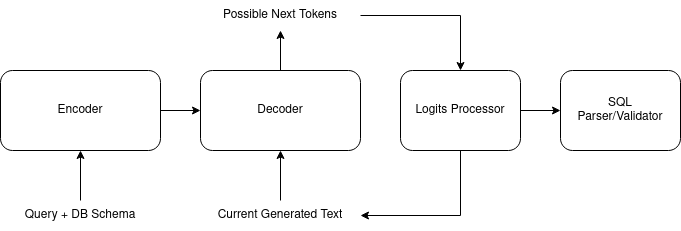
\includegraphics[width=\textwidth]{t5-transformer.drawio.png}
\caption{\label{fig:model} Model Overview}
\end{figure*}

The goal of this project was to assess the production viability of generating SQL from a natual language query for a common REST server. The model itself needed to be proven to be effective in a general sense and against a real database for a real use case. The integration of the model into the application also needed to account for the possibility of many concurrent users. It is also hoped that the model can be used in a general-purpose manner so that it can be adapted to whatever use case it might be beneficial for.

The \texttt{T5} model \citep{raffel2020exploring} is short for Text-to-Text Transfer Transformer and is one of the beginning auto-regressive Transformer models for text generation. It was created by Google in 2020 following \texttt{GPT-2} in 2019 \citep{radfordgpt2} and served as their solution for translation and summarization tasks in the wake of the shift to transformers from Recurrent Neural Networks. The \texttt{T5} has since been replaced at Google by \texttt{FLAN-T5} \citep{chung2022scaling} and \texttt{PaLM} \citep{chowdhery2022palm}, but still remains as one of the state of the art models used for Text-to-SQL generation.

Despite there being models that are technically better than the \texttt{T5} model, we still used it for our assessment because it has been proven to work for our needs. The major difference in our task versus the others in this space is that our demo application requires the generated SQL to target a predetermined table and produce a predetermined set of columns. This requirement is easily satisfied by an auto-regressive Transformer that is paired with a constrained decoder and is another reason the the \texttt{T5} model is a viable option for our needs.

% Evaluation (explain how you answered your question and how your evaluation substantiates that claim, also discuss the limitations of your work--what can you reasonably expect it to do and not to do)
\section{Evaluation} \label{sec:eval}


\subsection{Task \& Procedure}

\subsubsection{Model}

We started our efforts with a \texttt{T5} model that was already fine-tuned by the Picard project \citep{scholak2021picard}. This model was used because it is one of the state of the art models in this area of study and is easy to build off of due to its compatibility with Huggingface \citep{wolf2020huggingfaces}. We also benefitted from this model's database schema agnosticity because it expects the target database schema as an input and that meant that further fine-tuning to support a particular database is unnecessary. This is the main reason that no further fine-tuning was done.

We augmented this model by pairing it with a custom Huggingface Logits Processor that utilizes a \texttt{PyParsing} PostgreSQL SQL grammar \citep{githubPyparsing} to parse the generated SQL and ensure the chosen tokens contribute to a valid SQL output. This was done to implement a constrained decoder for our model and is useful because it helps ensure that the overall generated SQL is valid. We could have used Picard's Logits Processor, but chose not to because their solution utilized Haskell and thus would have been difficult to modify. Figure~\ref{fig:model} illustrates how the Transformer, Logits Processor and SQL parser work in tandem.

A constrained decoder approach is useful for text generation with Transformers that are meant for a specialized task like code generation. A model can be trained to do a lot of things, but it's debatable how perfect of a job it can do in all situations. A constrained decoder fills in the gaps by steering the text generation in the right direction. It can even be argued that a constrained decoder allows for a smaller model, with less parameters. Picard's constrained decoder for instance knows more details about the target database schema than what is provided in the inputs to the encoder and can thus make sure the proper operators and literals are used based on the type of table columns that they are being used alongside.

In addition to a custom Logits Processor, we also added a forced prefix to the generated SQL output by utilizing Huggingface's support for a restricted vocabulary. This was done to ensure that the generated SQL targeted the expected table and outputted the expected columns. Our demo application relied on this behavior due to the assumption that the generated SQL would always target a predetermined table and would return all of the columns related to that table. Our constrained decoder strategy likely wouldn't have been possible without the auto-regressive nature of our model and wouldn't have met our requirements for generating valid SQL that retrieves predetermined information.

For the general evaluation of this model we utilized the \texttt{Spider Text-to-SQL} dataset \citep{yu2019spider} to verify that the model by itself is capable of generating reasonable SQL results. This was done in a unit test environment.

We also relied on a human evaluation for our demo application as a whole. Refer to Figure~\ref{fig:architecture} for an idea of the overall architecture. This was necessary to evaluate how well our Text-to-SQL strategy worked against a real database for a real use case. Part of the evaluation was determining what was necessary to utilize the generated SQL for real database queries, while the other part was validating that the generated SQL made sense based on the natual language queries that we used for our movie database.

\begin{figure}
\centering
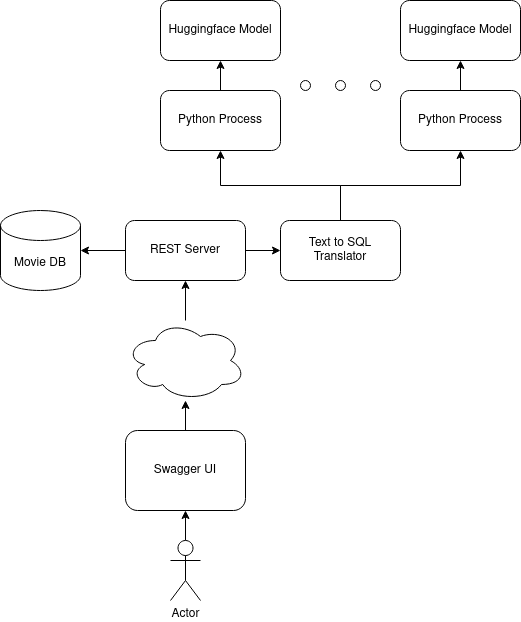
\includegraphics[width=0.5\textwidth]{demo-architecture.drawio.png}
\caption{\label{fig:architecture} Demo Architecture}
\end{figure}

\subsubsection{Framework}

The model was a core effort for this project, but the framework around that model is equally important. In order for the model to be useful in a production environment it needs to support multiple users to some degree. This ultimately needed to be a focus of the project to assess production viability.

The approaches explored for scalability included spawning Python processes with their own model based on the load of the application and utilizing batching for the queries. Figure~\ref{fig:architecture} illustrates the overall architecture for the demo application. The \texttt{Text to SQL Translator} piece was written to be a separate library that can be stood up on multiple computers if necessary and its main feature is that it spawns worker Python processes with our model based on the translation load. This was accomplished using Deep Java Library's model serving utility \citep{djlserving}.

DJL does a lot of things, but its serving utility claims to automatically support scaling up/down workers based on the load and dynamically batching requests. Although, these features weren't fully explored and evaluated in this project, we still have incorporated its usage into the overall project with the assumption that its features work as expected. More exploration is required for how this library can be configured to fully accomplish a production environment's scaling needs while taking to account excessive RAM usage of the models and ensuring batch sizes aren't too large.

\subsubsection{Metrics}

The various evaluation efforts used in this project required different metrics based on the strategies. The main evaluation utilized the Spider dataset to test the quality of the generated SQL. The results of that test were measured using a content overlap algorithm. We knew what sequence of tokens was expected to be in the output and also which tokens were actually present in the generated SQL output itself. This allowed us to calculate our accuracy as an overall percentage of the expected tokens that matched the actual results. A side effect of this strategy is that the expected queries with a high amount of tokens contributed more to the resulting percentage than expected queries with less tokens. In addition to the accuracy metric we also had a timer for measuring the duration of the SQL generation throughout the Spider evaluation.

\subsubsection{Results}

The final percentage that we achieved for the Spider dataset evaluation was about \texttt{61.2\%} and that again represents the percentage of the total expected tokens matching what was in the generated SQL. The Picard project was able to achieve a higher percentage than ours at \texttt{74.8\%}, but also had a much better constrained decoder implementation that took into account the actual data types of the columns in the target database schema. Their incremental parser was also probably better in general as well. Our accuracy however is still much better than our random baseline, which is practically \texttt{0\%} because it could be calculated using $\frac{1}{32,102}^{T}$ where $32,102$ is the size of our model's vocabulary and $T$ is the total number of expected tokens in the Spider dataset.

The other result we got from our evaluation was that the SQL generation takes a decent amount of time, ranging from two seconds to two minutes. It doesn't help that the test was done on a laptop CPU rather than a GPU, but we can at least note that most generations took under ten seconds. A machine with a GPU would likely yield a better result, but that's difficult to assume due to the sequential nature of an auto-regressive Transformer used for text generation.

The human evaluation of the overall demo application didn't necessarily have results that can be measured, but we have observed some interesting details and obstacles. Unlike the Spider evaluation, the demo application requires that the generated SQL has a predetermined set of column outputs and targets a particular table. In hindsight forcing a prefix worked, but also artificially gave the decoder some unintended cues towards what the rest of the SQL should include. With the anticipation that the generated SQL might generate a \texttt{JOIN} clause, the forced prefix included an alias to the main table that was to be queried. This resulted in almost all of the generated SQL containing a \texttt{JOIN} clause regardless of its actual necessity and usage in the rest of the query.

The actual quality of the generated SQL was also dependent on the natural lanuage query being descriptive enough so that the model was able to identify which columns were being referenced. Our model was not trained for the database that it was paired with. That resulted in some vague natural language queries not generating the intended SQL output. For example, we expected queries like ``Movies from 1955'' to generate SQL with a release year condition, but the model was unable to make the connection to the release year column and did not generate the condition. Natural language queries that included an explicit reference to the column like ``Movies released in 1955'' on the other hand would produce the expected SQL output.

In the development of the model, we have also observed that the model and SQL parser can sometimes get into states where they appear to ``argue'' with each other over what parts of the SQL is and isn't valid. This mostly occurs when incremental parsing is enabled instead of only parsing the generated SQL when an end token is encountered. The only explanation we have is that the parser isn't failing fast enough during the generation due to how lenient it was written in order to account for partial word token, which when observed by themselves may be seen as invalid. If the parser confirms that a partial word token is valid in one pass and then invalid when the next token completes the word, then it's believable that the generation process might get into this state of confusion. In these situations the generated SQL usually grows to be very large and appears to only stop when the configured maximum length is reached. In the context of the overall application, this results in a timeout and a failure to generate the SQL output.

% Implications (who would use your work? who does it affect? would it affect anyone in a negative way?)


%\begin{figure}
%\centering
%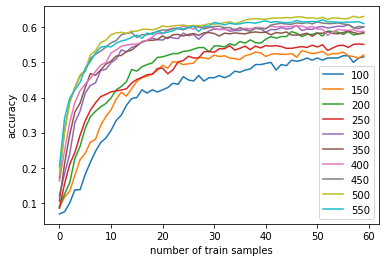
\includegraphics[width=0.5\textwidth]{figures/bert_funcs2emotions.png}
%\caption{\label{fig:results} Results for experiment 1: }
%\end{figure}

%Figure~\ref{fig:results} shows the results.

%Talk objectively about what you observe.


% Conclusion (bring everything together and write a concise take-home message)
\section{Conclusion}

%Explain more about your results and what they suggest.

The work explored in this project could easily be developed into a general-purpose library that has potential for being commonly used by any application that requires information to be retrieved from a database based on a user's needs. In the same way ORMs are designed to make database storage easier, this work makes the job of translating a user's request into the information that they wish to see easier. However, much like with ORMs this solution isn't going to replace the SQL that an expert is capable of writing for use cases that require efficient/performant queries and complete accuracy of the results. This approach will satisfy most of a user's needs, but will likely never be the right tool for every use case in the same way that the UDP protocol isn't the right tool for all communication.

\subsection{Implications}

%What do your results mean?

Based on our results we have found that our current model works, but requires additional training data or at the least documentation on how to write natural language queries that will produce the expected results. The need to have a table alias in the forced prefix does result in unintended \texttt{JOIN} clauses in the output, but just means that we need more training data to help prevent this situation. That is purely because we're using a pre-trained model that did not account for the way it is being used in this project.

The issue with vague natural language queries not generating the expected SQL is also a result of the pre-trained model that we're using. Our model was never trained on how to generate SQL for the database schema that we are using and it is working well despite that fact but is not perfect by any means. Additional training could help alleviate this, but there will always be natural language queries that cannot be accounted for and therefore some amount of documentation on how to use this tool effectively will probably be needed no matter what.

We also have learned from the results that our constrained decoder is not yet good enough. It does the job, but it does not adequately assist the model when being used in an incremental manner due to its inability to fail fast enough and it does not yet help the model use the correct operators and literals for the target column.


\subsection{Limitations}

%One limitation is ... the training data and test data could have some overlap ...

Overall limitations will likely always exist in our training data because it will not be easy to anticipate the usage of a general purpose SQL generator that can be used with any number of database schemas. Users will need to learn what keywords to use based on the database schema they are targeting. Database schemas will also need to use column and table names that are descriptive and relevant to how the users view the data that is stored. Both sides will need to be in alignment for the model to accurately generate SQL that does what is intended by the user.

There is also a potential problem with the overall performance of the SQL generation. An auto-regressive transformer has its benefits, but still requires the output to be sequentially generated and that will likely always cause a slowdown. Huggingface \cite{wolf2020huggingfaces} also lacks some features that could be used to help optimize this process, such as the ability to skip the decoding of certain tokens that the constrained decoder already expects in the output. If we already know what the prefix for the output should be, then using the decoder for those tokens is a waste of cycles. There are also other cases in SQL where only one possible token can come after the previous tokens and again using the decoder for these tokens is unnecessary. One example is the \texttt{ORDER BY} clause, which is made up of two keywords. If the ``ORDER'' keyword has been generated outside of quotes, then we can assume that it will be followed by the ``BY'' keyword.

\subsection{Future Work}

The steps required for this project to truly be considered viable for production uses will include the improvement of the constrained decoder, additional training for the model, and a focus on the scalability of the model. The constrained decoder will need a better parser that is able to fail as fast as possible and will also need better support for assuring that the model is correctly using the columns based on the database schema. \texttt{FLAN-T5} \citep{chung2022scaling} and \texttt{PaLM} \citep{chowdhery2022palm} will probably be better models than the dated \texttt{T5} model this project uses and will require additional training data to help ensure unnecessary \texttt{JOIN} clauses are not added to the SQL output. Scalability will also need to be explored and tested in more detail so that this model is able to handle a large amount of concurrent users.

The parser of the constrained decoder in particular is a difficult challenge because the model doesn't generate complete words with each pass through the decoder. The most basic conventional parsers available expect to parse entire words, one at a time, and in most cases a grammar's tokens are made up of multiple sub-tokens or literals. It's difficult to determine if the next token generated by our model is invalid without taking into account what will come after it. There is potentially a solution on how to make the model and a special parser work well together.

One idea we have is for the model to be trained to output a tree of grammar rules that can directly be used by a specialized PEG parser to very quickly determine whether the output is valid or invalid. This sort of strategy would effectively train the model to know about its target grammar instead of relying on a more complicated textual representation where the grammar is implicitly utilized. This effort would require a special dataset as well to adequately evaluate its performance, but should be possible. Another result would be that the specialized parser would also be able to be loaded with knowledge of the database schema that it is targeting and would be able to make better decisions on how the generated output should be altered to correctly utilize the columns in the target tables.

% Attached is an example submission that is worth emulating (you are not required to use multiple columns)


% Entries for the entire Anthology, followed by custom entries
\bibliography{custom}

% \appendix

% \section{Example Appendix}
% \label{sec:appendix}

% This is a section in the appendix.

\end{document}
